\begin{figure}[h]
  \centering
  \begin{subfigure}[b]{0.32\textwidth}
    \centering
    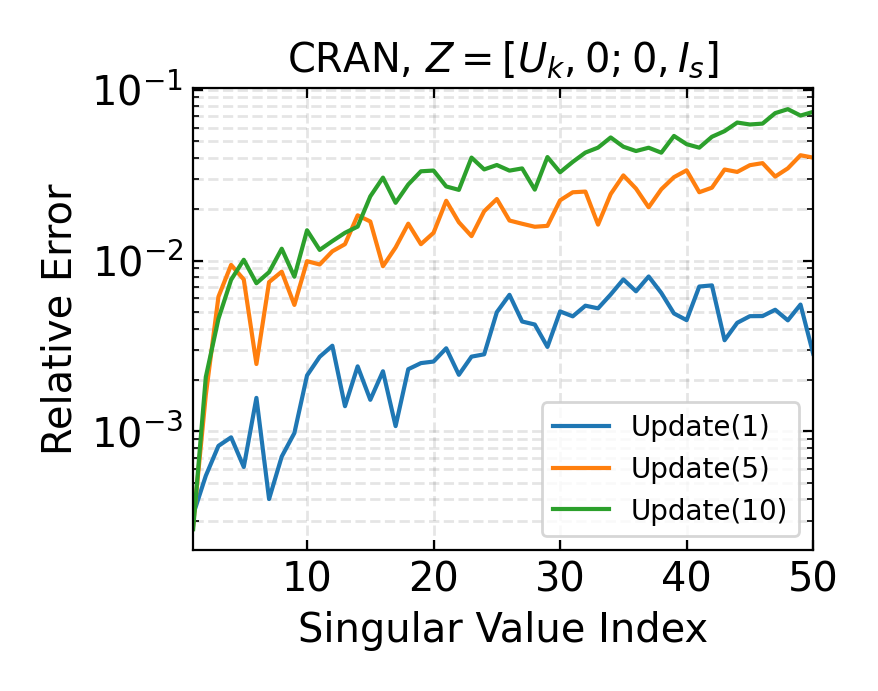
\includegraphics[width=\textwidth]{../openreview/figures/report_figures/CRAN_zha-simon_n_batches_10_k_dims_50_rel_err.png}
    \caption{CRAN relative error (Alg. 2.1)}
  \end{subfigure}
  \hfill
  \begin{subfigure}[b]{0.32\textwidth}
    \centering
    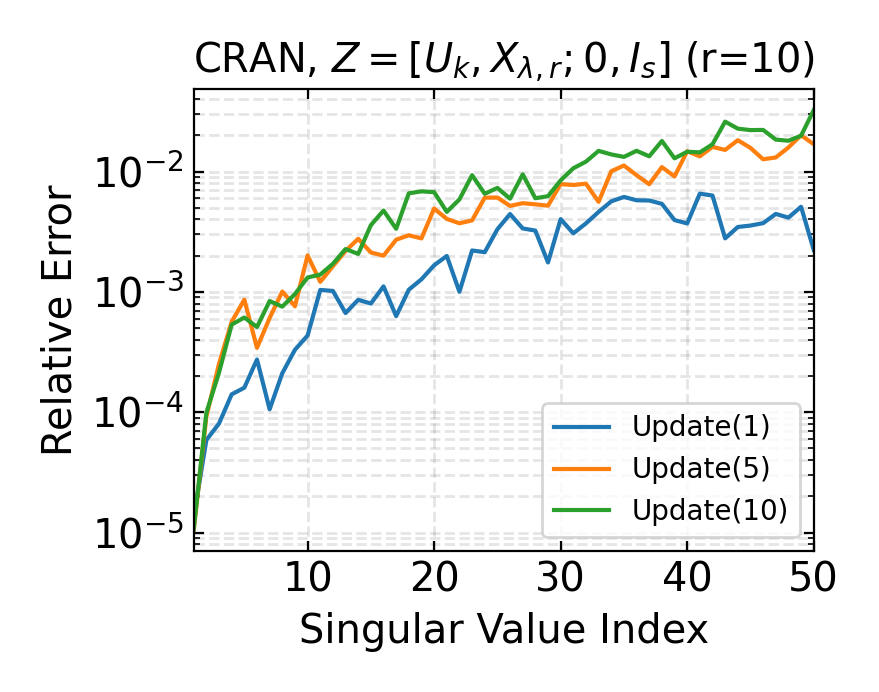
\includegraphics[width=\textwidth]{../openreview/figures/report_figures/CRAN_bcg_n_batches_10_k_dims_50_rval_10_rel_err.png}
    \caption{CRAN relative error (Alg. 2.2)}
  \end{subfigure}
  \hfill
  \begin{subfigure}[b]{0.32\textwidth}
    \centering
    \includegraphics[width=\textwidth]{../openreview/figures/report_figures/CRAN_frequent-directions_n_batches_10_k_dims_50_rel_err.png}
    \caption{CRAN relative error (FD)}
    \label{fig:cran_rel_err_fd}
  \end{subfigure}
  %
  \begin{subfigure}[b]{0.32\textwidth}
    \centering
    \includegraphics[width=\textwidth]{../openreview/figures/report_figures/CRAN_zha-simon_n_batches_10_k_dims_50_res_norm.png}
    \caption{CRAN residual norm (Alg. 2.1)}
  \end{subfigure}
  \hfill
  \begin{subfigure}[b]{0.32\textwidth}
    \centering
    \includegraphics[width=\textwidth]{../openreview/figures/report_figures/CRAN_bcg_n_batches_10_k_dims_50_rval_10_res_norm.png}
    \caption{CRAN residual norm (Alg. 2.2)}
  \end{subfigure}
  \hfill
  \begin{subfigure}[b]{0.32\textwidth}
    \centering
    \includegraphics[width=\textwidth]{../openreview/figures/report_figures/CRAN_frequent-directions_n_batches_10_k_dims_50_res_norm.png}
    \caption{CRAN residual norm (FD)}
    \label{fig:cran_res_norm_fd}
  \end{subfigure}
  \caption{Relative errors and residual norms at $\phi=1,5,10$ for CRAN with Algorithm 2.1, Algorithm 2.2, and FD.}
  \label{fig:cran_relerr_resnorm}
\end{figure}
